\documentclass[11pt]{article}
\usepackage{setspace}
\usepackage{fullpage}
\usepackage{pslatex}
\usepackage{pgfplots}
\pgfplotsset{
	compat=1.4}
\usepackage{tikz}
\usetikzlibrary{shapes,arrows}
\let\word=\textit
\begin{document}
\begin{figure}[htb]
\centering
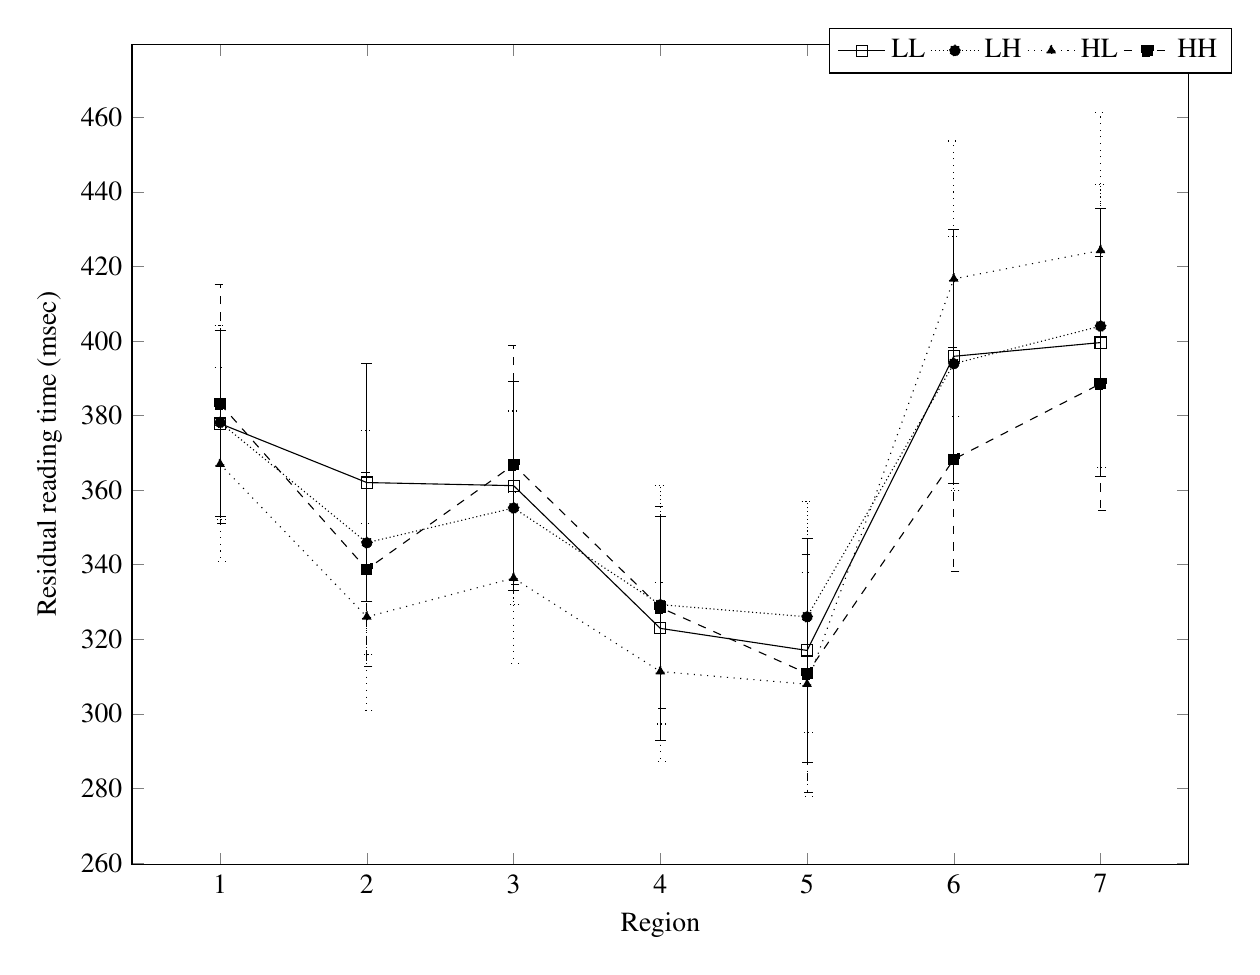
\begin{tikzpicture}
\begin{axis}[
	width=15cm, height=12cm,
	legend style={at={(0.85,1.02)},
	anchor=north,legend columns=-1},
	ylabel={Residual reading time (msec)},
	xlabel={Region},
	symbolic x coords={1, 2, 3, 4, 5, 6, 7},
    	xtick=data,
]
\addplot[
		mark=square,
		error bars/.cd,
		error bar style={color=black},
		y dir=both,
		y explicit
] 
	coordinates {(1, 377.8485 ) +- ( 25 , 25 )(2, 362.0291 ) +- ( 32 , 32 )(3, 361.2019 ) +- ( 28 , 28 )(4, 322.9233 ) +- ( 30 , 30 )(5, 317.007 ) +- ( 30 , 30 )(6, 395.8915 ) +- ( 34 , 34 )(7, 399.5707 ) +- ( 36 , 36 )};
\addplot[
		mark=*,
		densely dotted,
		error bars/.cd,
		error bar style={color=black},
		y dir=both,
		y explicit
] 
	coordinates {(1, 378.1518 ) +- ( 26 , 26 )(2, 345.8896 ) +- ( 30 , 30 )(3, 355.2114 ) +- ( 26 , 26 )(4, 329.2884 ) +- ( 32 , 32 )(5, 326.0267 ) +- ( 31 , 31 )(6, 393.9068 ) +- ( 34 , 34 )(7, 403.9804 ) +- ( 38 , 38 )};
\addplot[
		mark=triangle*,
		dotted,
		error bars/.cd,
		error bar style={color=black},
		y dir=both,
		y explicit
] 
	coordinates {(1, 366.9766 ) +- ( 26 , 26 )(2, 326.0031 ) +- ( 25 , 25 )(3, 336.3977 ) +- ( 23 , 23 )(4, 311.3395 ) +- ( 24 , 24 )(5, 307.9527 ) +- ( 30 , 30 )(6, 416.6444 ) +- ( 37 , 37 )(7, 424.2883 ) +- ( 37 , 37 )};
\addplot[
		mark=square*,
		dashed,
		error bars/.cd,
		error bar style={color=black},
		y dir=both,
		y explicit
] 
	coordinates {(1, 383.1588 ) +- ( 32 , 32 )(2, 338.7696 ) +- ( 26 , 26 )(3, 366.7928 ) +- ( 32 , 32 )(4, 328.5057 ) +- ( 27 , 27 )(5, 310.8256 ) +- ( 32 , 32 )(6, 368.2896 ) +- ( 30 , 30 )(7, 388.5395 ) +- ( 34 , 34 )};
\legend{LL,LH,HL,HH}
\end{axis}
\end{tikzpicture}
\caption{Mean residual reading times for all sentence regions}
\end{figure}
\end{document}